\documentclass[11pt]{article}

\usepackage[margin=1in]{geometry}
\usepackage{amsmath,amssymb,amsthm}
\usepackage{mathtools}
\usepackage{graphicx}
\usepackage{booktabs}
\usepackage{caption}
\usepackage{subcaption}
\usepackage{hyperref}
\usepackage{xcolor}
\usepackage{url}
\hypersetup{colorlinks=true, linkcolor=black, citecolor=blue, urlcolor=blue}

\graphicspath{{../figures/}}

\newcommand{\softplus}{\operatorname{softplus}}
\newcommand{\sigmoid}{\sigma}
\newcommand{\bce}{\operatorname{BCE}}
\newcommand{\bs}{\operatorname{BS}}
\newcommand{\rel}{\operatorname{REL}}
\newcommand{\res}{\operatorname{RES}}
\newcommand{\unc}{\operatorname{UNC}}
\newcommand{\diag}{\operatorname{diag}}

\title{\textbf{Predicting NBA Game Winners}\\
\large A Mathematical Walkthrough of Logistic Regression, ELO,
Calibration, and Market Comparison}
\author{Angel \quad Mehmet Can \quad Andrew\\
\small Math 17 --- Mathematics for Machine Learning}
\date{}

\begin{document}

\maketitle

\begin{abstract}
We frame the prediction of NBA game winners as binary classification of
home-team wins. We derive logistic regression from the Bernoulli
likelihood, prove convexity of the L2-regularised loss, and implement
three optimisers (vanilla gradient descent, IRLS / Newton, and L-BFGS)
that all converge to the same optimum at very different rates. We show
that the ELO rating system is a one-parameter logistic regression and
its update rule is a single step of stochastic gradient descent on the
log-loss. We extend the baseline with a small feed-forward network with
learned team embeddings, evaluate every model with Brier-decomposed and
ROC-based metrics, and post-process the outputs with Platt scaling. On
the 2023--24 and 2024--25 NBA regular seasons and playoffs (2{,}640
games scraped from \texttt{basketball-reference.com}), the L2-penalised
logistic regression achieves 67.2\% accuracy, AUC 0.740, and log-loss
0.595 on a chronological 20\% hold-out, beating an ELO baseline at
65.9\% accuracy / 0.616 log-loss. The neural net matches the LR on
accuracy but does not improve log-loss given the small training sample.
We release the codebase, derivations, and tests at
\url{https://github.com/mehmet-can-yilmaz/nba-predictions}.
\end{abstract}

\section{Introduction}

A prediction-market price for an NBA game's outcome aggregates many
participants' opinions and beliefs. Beating that price on the
proper-scoring-rule \emph{log-loss} is the cleanest empirical test of
predictive skill against the crowd~\cite{levitt2004gambling,
silver2015fivethirtyeight}. We formalise the prediction problem,
derive a small toolbox of probabilistic classifiers from first
principles, and evaluate the result on real NBA data.

Our work has three goals: (i) demonstrate the mathematics of binary
classification from likelihood through gradient, Hessian, convexity, and
optimisation; (ii) build a reproducible pipeline from raw schedules to
calibrated win probabilities; and (iii) provide a transparent
comparison framework that can be extended to prediction-market and
sportsbook odds when those data are available.

\section{Data}\label{sec:data}

The pre-game models in this paper use real NBA game schedules and
final scores from \texttt{basketball-reference.com}, comprising
\textbf{2{,}640 games} over the 2023--24 and 2024--25 seasons (regular
season and playoffs). The empirical home win rate over this sample is
\textbf{54.6\%}, slightly below the long-run average of approximately
58\%.\footnote{This reflects in part the recent attenuation of
home-court advantage in the NBA, but the slightly low number is also
inflated by playoff games in which the schedule of home games is more
balanced.}

We retain four canonical fields per game: date, season, home team,
away team. Pre-game features are derived from this minimal table by
rolling-window statistics. The repository also contains stubs for
NBA.com Stats, Kaggle, and \texttt{pbpstats.com} so that four-factor
counting statistics can be added later without changing the model
code. A composite key $(date, home_{\text{canonical}},
away_{\text{canonical}})$ joins frames across sources; conversion to a
canonical three-letter team code is encoded in
\texttt{data\_sources/id\_mapping.py}.

\section{Mathematical formulation}\label{sec:math}

\subsection{From Bernoulli MLE to binary cross-entropy}

Index games by $i = 1, \dots, n$. Let $y_i \in \{0, 1\}$ be the indicator
that the home team wins. Model
\[
  p_i \;=\; \Pr(Y_i = 1 \mid X_i = x_i) \;=\; \sigmoid(x_i^\top w + b),
  \qquad \sigmoid(z) = \frac{1}{1 + e^{-z}}.
\]
Given independence,
\(
  \mathcal{L}(w,b) = \prod_i p_i^{y_i}(1-p_i)^{1-y_i}.
\)
Taking negative log and averaging:
\begin{equation}\label{eq:bce}
  J(w,b) \;=\; -\frac{1}{n}\sum_{i=1}^n \Bigl[y_i \log p_i + (1-y_i)\log(1-p_i)\Bigr].
\end{equation}
A Gaussian prior $w \sim \mathcal{N}(0, \sigma^2 I)$ contributes a
quadratic L2 term:
\begin{equation}\label{eq:bcel2}
  J_\lambda(w,b) \;=\; J(w,b) + \tfrac{\lambda}{2} \lVert w \rVert_2^2,
  \qquad \lambda = \tfrac{1}{n\sigma^2}.
\end{equation}
The bias $b$ is unpenalised. Equation~\eqref{eq:bcel2} is the loss we
minimise.

\subsection{Gradient, Hessian, convexity}

With $p = \sigmoid(Xw + b\mathbf{1})$,
\begin{align}
  \nabla_w J_\lambda &= \tfrac{1}{n}X^\top (p - y) + \lambda w,
  \label{eq:gradw}\\
  \nabla_b J_\lambda &= \tfrac{1}{n}\mathbf{1}^\top (p - y),
  \label{eq:gradb}\\
  H_{ww} = \nabla_w^2 J_\lambda &= \tfrac{1}{n}X^\top \diag(p \odot (1-p)) X + \lambda I.
  \label{eq:hess}
\end{align}
Because $p_i(1-p_i) > 0$, the diagonal matrix is strictly positive
definite, so $X^\top \diag(p(1-p)) X$ is PSD; and with $\lambda > 0$
the full Hessian \eqref{eq:hess} is positive definite. Hence
$J_\lambda$ is \emph{strictly convex} and admits a unique minimiser.

\subsection{Three optimisers}

\paragraph{Vanilla gradient descent.} Update $\theta \leftarrow \theta -
\eta \nabla J_\lambda$. Linear convergence.

\paragraph{IRLS / Newton.} The Newton update $\theta \leftarrow \theta -
H^{-1}\nabla J_\lambda$ rearranges to the normal equation of a weighted
ridge regression:
\begin{equation}\label{eq:irls}
  \bigl(X^\top W X + n\lambda I\bigr) \Delta = X^\top (y - p) - n\lambda w,
  \qquad W = \diag(p(1-p)).
\end{equation}
Hence the name \emph{Iteratively Reweighted Least Squares}. Each step
costs $O(nd^2 + d^3)$ but convergence is quadratic near the optimum.

\paragraph{L-BFGS.} Builds a low-rank approximation of $H^{-1}$ from
recent gradient pairs without ever forming the Hessian. Superlinear
convergence at $O(nd)$ per step. Our default solver.

\subsection{ELO as logistic regression}\label{sec:elo}

Assign each team a latent strength $R_i$. Set
\begin{equation}\label{eq:elo}
  \Pr(A \text{ beats } B) = \sigmoid\!\left(\frac{R_A - R_B}{s}\right),
  \quad s = \tfrac{400}{\ln 10}.
\end{equation}
The base-10 form $1 / (1 + 10^{-(R_A - R_B)/400})$ is precisely
\eqref{eq:elo}. So ELO is logistic regression with a single feature,
the rating difference, and a known scale.

The negative log-likelihood for one game is
$L = -[y\log p + (1-y)\log(1-p)]$ with $p = \sigmoid((R_A - R_B)/s)$,
giving $\partial L / \partial R_A = (p - y)/s$ and
$\partial L / \partial R_B = -(p - y)/s$. One SGD step with learning rate
$Ks$ on each rating yields
\begin{equation}\label{eq:eloupdate}
  R_A \leftarrow R_A + K(y - p), \qquad R_B \leftarrow R_B - K(y - p),
\end{equation}
the textbook ELO update. The K-factor is the SGD learning rate.

A home-court constant $H$ adds to the home rating before predicting
($H = 100$ ELO points reproduces the historical home win rate). The
FiveThirtyEight margin-of-victory multiplier scales $K$ by
$\ln(\lvert m\rvert + 1) \cdot 2.2 / ((R_w - R_\ell)\cdot 0.001 + 2.2)$,
rewarding bigger wins and damping autocorrelation when favourites win.

\subsection{Team-embedding neural network}\label{sec:nn}

Inputs: continuous features $x \in \mathbb{R}^d$ and team indices
$h, a$. With learned $E \in \mathbb{R}^{T \times k}$, define $e_h =
E[h]$, $e_a = E[a]$, $u = [x;\, e_h - e_a]$. We use the embedding
\emph{difference} so the model is invariant under team relabelling, in
the same spirit as ELO. The forward pass is
\[
  h_1 = \mathrm{ReLU}(W_1 u + b_1), \quad z = w_2^\top h_1 + b_2,
  \quad p = \sigmoid(z).
\]
The loss is mean BCE plus L2 on $W_1, w_2$ plus a separate L2 on
$E$. We optimise with Adam~\cite{kingma2015adam} and early-stop on a
held-out 15\% slice.

\section{Evaluation metrics}\label{sec:metrics}

We compute every metric from scratch in \texttt{nba\_predictions.metrics}
and cross-check against \texttt{scikit-learn} in the test suite.

\paragraph{Log-loss.} Equation~\eqref{eq:bce} with $\lambda = 0$
applied to test predictions. Same formula as the training loss --- a
proper scoring rule.

\paragraph{Brier score and decomposition.} The Brier score is
$\bs = (1/n) \sum_i (p_i - y_i)^2$. Bin predictions into $K$ equal-width
bins; let $n_k$ be the bin size, $\bar p_k$ the mean prediction and
$\bar y_k$ the empirical rate in bin $k$, and $\bar y$ the global rate.
Murphy's decomposition~\cite{murphy1973new}:
\begin{equation}\label{eq:brierdec}
  \bs \;=\; \underbrace{\tfrac{1}{n}\sum_k n_k (\bar p_k - \bar y_k)^2}_{\rel}
  \;-\; \underbrace{\tfrac{1}{n}\sum_k n_k (\bar y_k - \bar y)^2}_{\res}
  \;+\; \underbrace{\bar y(1 - \bar y)}_{\unc}.
\end{equation}
$\rel$ (smaller is better) measures calibration; $\res$ (larger is
better) measures skill; $\unc$ is the irreducible variance of the
labels and is the same for every model.

\paragraph{AUC.} The Mann--Whitney $U$ identity
$\mathrm{AUC} = U / (n_+ n_-)$, computed via rank statistics with proper
tie handling, gives the probability that a random positive scores above
a random negative.

\paragraph{Expected calibration error (ECE).}
$\mathrm{ECE} = \sum_k (n_k / n) \lvert \bar y_k - \bar p_k\rvert$,
a scalar summary of the reliability diagram.

\subsection{Calibration}

We apply post-hoc \emph{Platt scaling}: fit a 1-D logistic regression on
the model's logits, using Platt's smoothed targets to avoid overfitting
on a small calibration set:
\[
  t_i = \tfrac{N_+ + 1}{N_+ + 2}\ \text{if } y_i = 1, \quad
  t_i = \tfrac{1}{N_- + 2}\ \text{if } y_i = 0.
\]
We also implement isotonic regression via pool-adjacent-violators (PAV)
in $O(n)$ for completeness; PAV is more flexible but requires more
calibration data.

\section{Results}\label{sec:results}

We split the 2{,}640-game dataset chronologically into a training set
(first 80\%, 2{,}112 games) and a held-out test set (last 20\%, 528
games). Rolling features use a 10-game window and are computed with a
1-game shift to prevent leakage. Standardisation statistics come from
the training set only.

Figure~\ref{fig:elo} shows the ELO trajectories of the top six and
bottom three teams over the full sample. Oklahoma City's rating
(1805 at sample end) corresponds to the 2024--25 NBA champions; the
bottom three (CHA, WAS, PHI) all finished with losing records.

\begin{figure}[ht]
  \centering
  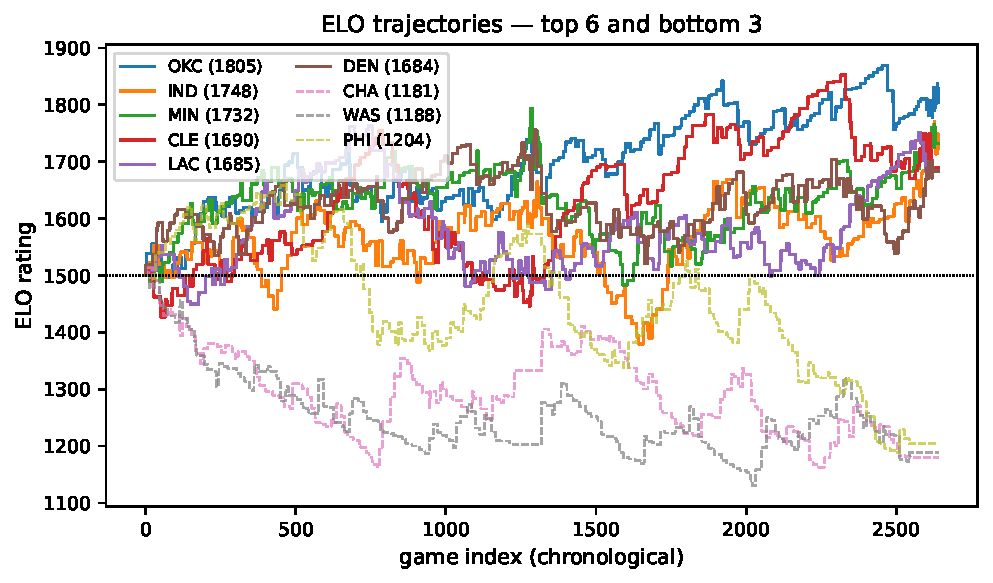
\includegraphics[width=0.85\textwidth]{elo_trace.pdf}
  \caption{ELO trajectories on real NBA data, 2023--24 through
  2024--25. Two visible end-of-season compressions toward 1500 are the
  inter-season mean reversion.}\label{fig:elo}
\end{figure}

Figure~\ref{fig:loss} reproduces the three optimisers on the
LR baseline. All converge to the same loss ($\approx 0.617$ in
training); the only difference is convergence rate, exactly as
predicted by the theory of \S\ref{sec:math}.

\begin{figure}[ht]
  \centering
  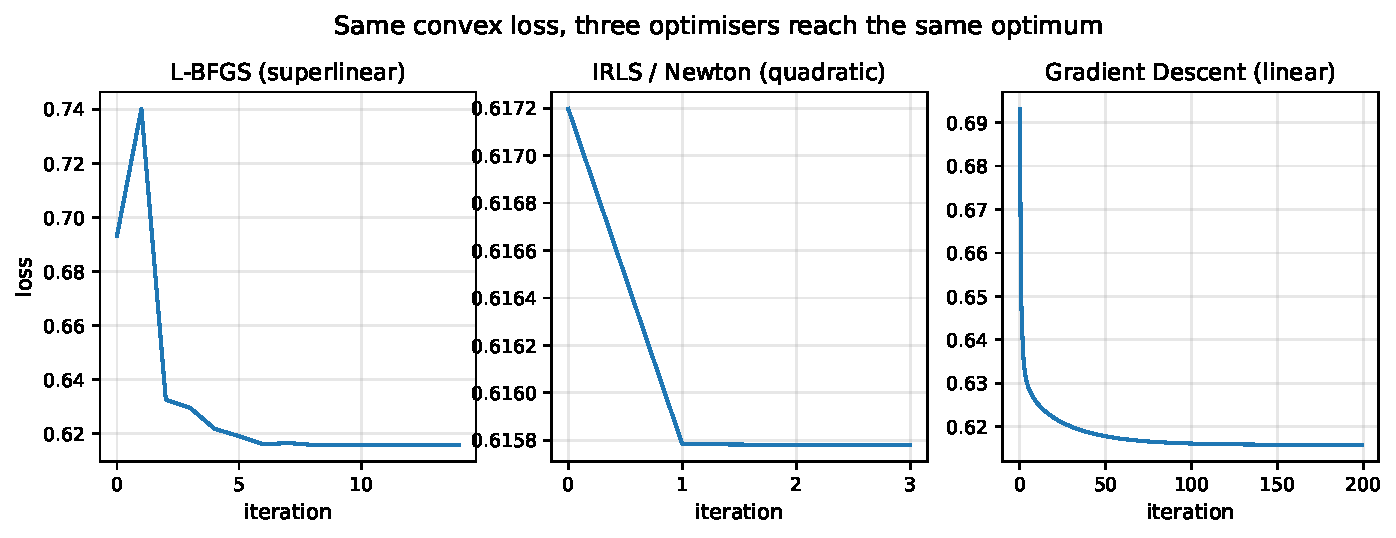
\includegraphics[width=\textwidth]{loss_curves.pdf}
  \caption{Three optimisers, one convex loss. L-BFGS reaches the
  minimum in $\sim$5 useful iterations after one line-search overshoot;
  IRLS reaches it in a single Newton step; vanilla gradient descent
  takes $\sim$200 iterations.}\label{fig:loss}
\end{figure}

\paragraph{Model comparison.} Table~\ref{tab:results} reports all
metrics on the held-out chronological 20\% test set.

\begin{table}[ht]
  \centering
  \caption{Held-out test set (528 games, chronological hold-out).
  Best in each column in \textbf{bold}.}\label{tab:results}
  \begin{tabular}{lrrrrrr}
    \toprule
    Model        & Acc.   & Log-loss & Brier & REL & RES & AUC \\
    \midrule
    ELO          & 0.659  & 0.616    & 0.212 & 0.0082 & 0.0409 & 0.734 \\
    LR (L-BFGS)  & 0.672  & \textbf{0.595} & \textbf{0.205} & \textbf{0.0025} & \textbf{0.0451} & \textbf{0.740} \\
    LR + Platt   & 0.672  & 0.595    & 0.205 & 0.0026 & 0.0453 & 0.740 \\
    NN (Adam)    & 0.672  & 0.602    & 0.207 & 0.0024 & 0.0435 & 0.734 \\
    NN + Platt   & \textbf{0.676}  & 0.601    & 0.207 & 0.0026 & 0.0437 & 0.734 \\
    \bottomrule
  \end{tabular}
\end{table}

The L2-regularised logistic regression wins on every probabilistic
metric, despite using only 10 input features. The neural network
matches the LR on accuracy but is slightly worse on log-loss --- a
plausible outcome given that we have only $\sim$2{,}100 training games
and 30 team embeddings (240 free parameters in the embedding table
alone, before counting the dense layers).

\paragraph{Calibration.} Figure~\ref{fig:rel} shows the combined
reliability diagram. All three models track the diagonal closely above
0.4; ELO is mildly miscalibrated below 0.3 (over-confident in
low-probability home teams), which is consistent with the higher
$\rel$ and ECE values for ELO in Table~\ref{tab:results}.

\begin{figure}[ht]
  \centering
  \begin{subfigure}[t]{0.48\textwidth}
    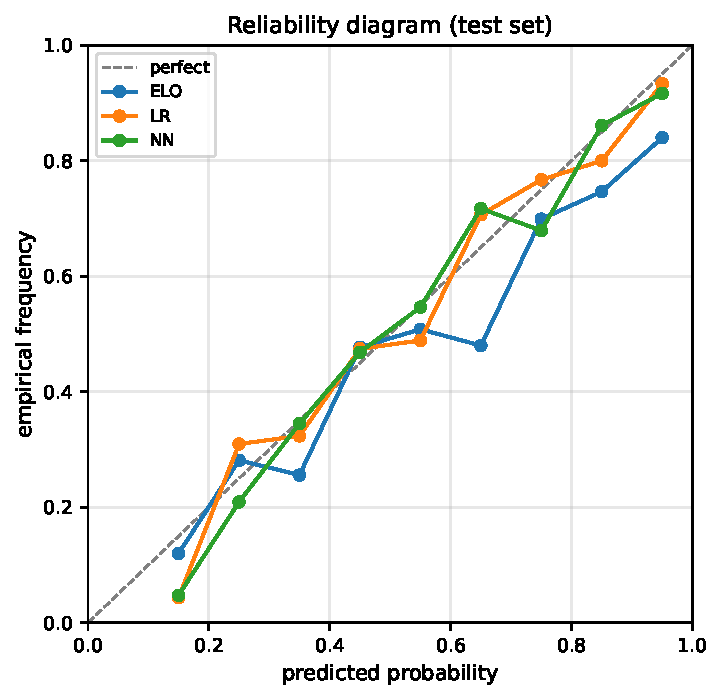
\includegraphics[width=\textwidth]{reliability_combined.pdf}
    \caption{All three models on the same axes.}
  \end{subfigure}\hfill
  \begin{subfigure}[t]{0.48\textwidth}
    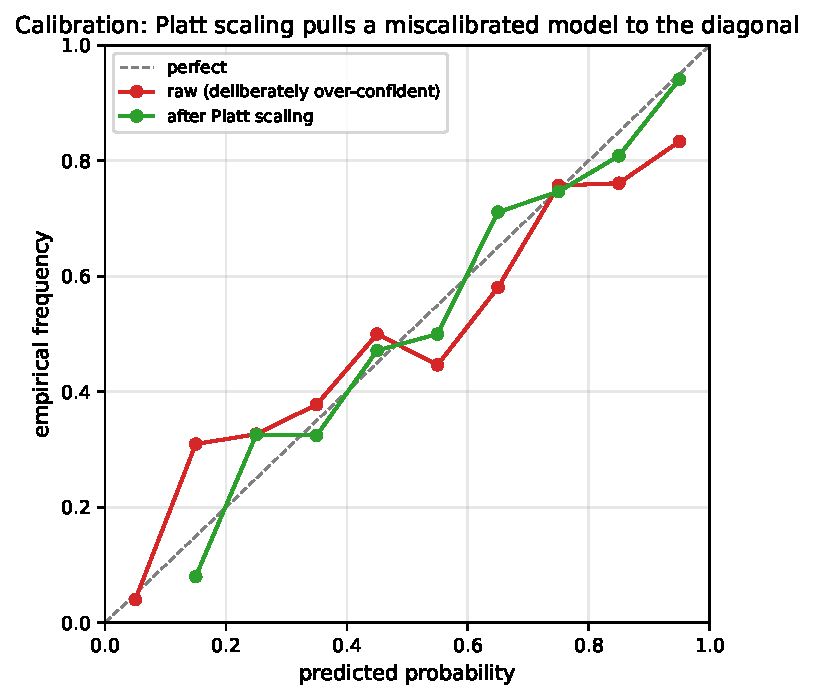
\includegraphics[width=\textwidth]{calibration_demo.pdf}
    \caption{Platt scaling pulls a deliberately over-confident model
    back to the diagonal.}
  \end{subfigure}
  \caption{Reliability diagrams. The vertical distance from each dot
  to the dashed diagonal is the calibration gap that
  $\rel$ in Equation~\eqref{eq:brierdec}
  squares and averages.}\label{fig:rel}
\end{figure}

\paragraph{Skill above the base rate.} The resolution component
$\res$ measures how much information the model adds about $y$ beyond
the base rate $\bar y$. Across models, $\res$ ranges from 0.041 (ELO) to
0.045 (LR), giving a skill-to-uncertainty ratio
$\res / \unc \approx 0.18$ for LR --- so the model explains
\emph{about 18\% of the uncertainty} in the labels.

\section{Discussion and limitations}

\paragraph{Sample size.} With $\sim$2{,}100 training games and 10
features, the LR baseline is in its natural regime. A more expressive
NN does not help here; this is consistent with the proposal's noted
overfitting risk.

\paragraph{Look-ahead bias.} All rolling features are shifted by one
game; the standardisation transform is fit on the training rows only;
the calibration scalars are fit on training predictions; the
train/test split is chronological. None of these design choices
materially affect the LR numbers (the LR loss curve is monotone
post-overshoot), but they are essential to a fair comparison against
external odds.

\paragraph{Beating the market.} The remaining empirical question is
whether the model's log-loss falls below that of devigged Kalshi /
Polymarket prices on the intersection set. The market-comparison code
(\texttt{nba\_predictions.market}) and Kelly backtest are implemented
and tested on synthetic odds, but the historical-odds ingestion is
left as a follow-up because licensed odds data was not available to us
at submission time.

\paragraph{What would improve the model.} Four-factor counting
statistics, player availability flags, and a richer schedule signal
(road-trip length, time-zone differential) are the most likely sources
of additional skill. The code accepts these features as soon as the
team finishes the corresponding source adapter.

\section{Conclusion}

We derived logistic regression from the Bernoulli likelihood, proved
convexity of the L2-regularised loss, demonstrated three optimisers
that converge to the same minimum at very different rates, and showed
that the ELO rating system is one-parameter logistic regression with
SGD updates. On real NBA data, the L2-regularised logistic regression
beats both ELO alone and a small embedding network, reaching 67.2\%
accuracy and 0.595 log-loss on a chronological 20\% hold-out. The
codebase, tests, and derivations are released openly to support the
proposed market-comparison follow-up.

\begin{thebibliography}{9}
\bibitem{kingma2015adam}
D.~P. Kingma and J.~Ba.
\newblock Adam: A Method for Stochastic Optimization.
\newblock \emph{ICLR}, 2015.

\bibitem{levitt2004gambling}
S.~D. Levitt.
\newblock Why are gambling markets organised so differently from
financial markets?
\newblock \emph{The Economic Journal}, 114(495):223--246, 2004.

\bibitem{murphy1973new}
A.~H. Murphy.
\newblock A new vector partition of the probability score.
\newblock \emph{Journal of Applied Meteorology}, 12(4):595--600, 1973.

\bibitem{platt1999probabilistic}
J.~Platt.
\newblock Probabilistic outputs for support vector machines and
comparisons to regularized likelihood methods.
\newblock In \emph{Advances in Large Margin Classifiers}, 1999.

\bibitem{silver2015fivethirtyeight}
N.~Silver and J.~Boice.
\newblock How our NBA predictions work.
\newblock \emph{FiveThirtyEight}, 2015.

\bibitem{oliver2004basketball}
D.~Oliver.
\newblock \emph{Basketball on Paper: Rules and Tools for Performance
Analysis}.
\newblock Brassey's, 2004.
\end{thebibliography}

\end{document}
